\documentclass{article}
\usepackage[utf8]{inputenc}

\usepackage{amsthm}
\usepackage{amssymb}
\usepackage{amsmath}
\usepackage{color}

\usepackage{hyperref}
\usepackage{url}
\usepackage{times}
\usepackage[algo2e]{algorithm2e}

%\usepackage{fullpage}
%\usepackage{amsmath,amsfonts,amsthm,amssymb}
\usepackage{bbm}
\usepackage{graphics, graphicx, xcolor}
\usepackage{enumitem}
%\usepackage{verbatim}		% for misc commenting, etc.
\usepackage{stmaryrd}
\usepackage{float}
\usepackage[mathscr]{euscript}


\usepackage{geometry}
%% \geometry{a4paper,
%%   total={170mm,220mm},
%%   marginparwidth=80mm,
%% left=5mm,
%% right=85mm,
%% top=20mm,
%% }

% For algorithms
\usepackage{algorithm}
\usepackage{algorithmic}


\title{Active learning using muffler}
\author{Akshay Balsubramani, Yoav Freund, Shay Moran}
\date{November 2016}

\newtheorem{theorem}{Theorem}[section]
\newtheorem{corollary}{Corollary}[theorem]
\newtheorem{lemma}[theorem]{Lemma}
\newtheorem{assumption}[theorem]{assumption}
\newtheorem{definition}[theorem]{Definition}

\newtheorem{thm}{Theorem}%[section]
\newtheorem{lem}[thm]{Lemma}
\newtheorem{prop}[thm]{Proposition}
\newtheorem{cor}[thm]{Corollary}
\newtheorem{conj}[thm]{Conjecture}
\newtheorem{obs}[thm]{Observation}
\newtheorem{defn}[thm]{Definition}
\newtheorem{alg}{Algorithm}
\newtheorem{ass}{Assumption}
\newtheorem{examp}{Example}
\newtheorem{property}{Property}
\setcounter{MaxMatrixCols}{20}

\DeclareMathOperator{\id}{id}
\DeclareMathOperator{\tr}{tr}
\DeclareMathOperator*{\argmin}{arg\,min}
\DeclareMathOperator*{\argmax}{arg\,max}
\DeclareMathOperator{\sgn}{sgn}
\DeclareMathOperator{\Prtxt}{Pr}
\DeclareMathOperator{\var}{var}
\DeclareMathOperator{\poly}{poly}
\DeclareMathOperator{\polylog}{polylog}

\newcommand{\err}{\mbox{err}}
\newcommand{\X}{{\cal X}}
\newcommand{\Y}{{\cal Y}}
\newcommand{\D}{{\cal D}}
\newcommand{\B}{{\cal B}}
\newcommand{\x}{\vec{x}}
\newcommand{\y}{\vec{y}}
\newcommand{\vv}{\vec{v}}
\newcommand{\cc}{\vec{c}}

\newcommand{\K}{{\cal K}}
\newcommand{\restrictedto}{\triangleright}
\renewcommand{\SS}{{\cal S}} % Specialists
\newcommand{\CC}{{\cal C}}  % constraints

\newcommand{\outcome}{z}
\newcommand{\empoutcome}{\hat{\outcome}}
\newcommand{\polarity}{p}

\newcommand{\bd}[1]{\mathbf{#1}}  % for bolding symbols
\newcommand{\RR}{\mathbb{R}}      % Real numbers
\newcommand{\ZZ}{\mathbb{Z}}      % Integers
\newcommand{\NN}{\mathbb{N}}      % natural numbers
\newcommand{\RP}{\mathbb{RP}}      % real projective space
\newcommand{\Sp}{\mathbb{S}}
\newcommand{\HH}{\mathbb{H}}
\newcommand{\col}[1]{\left[\begin{matrix} #1 \end{matrix} \right]}
\newcommand{\comb}[2]{\binom{#1^2 + #2^2}{#1+#2}}
\newcommand{\vnorm}[1]{\left\lVert#1\right\rVert} % vector norm
\newcommand{\bfloor}[1]{\left\lfloor#1\right\rfloor} % floor function
\newcommand{\bceil}[1]{\left\lceil#1\right\rceil} % ceiling function
\newcommand{\ifn}{\mathbf{1}} % indicator function for sets
\newcommand{\EV}{\mathbb{E}} % expected value operator
\newcommand{\evp}[2]{\mathbb{E}_{#2} \left[#1\right]} % expected value operator
\newcommand{\abs}[1]{\left| #1 \right|}
\newcommand{\pr}[1]{\Prtxt \left(#1\right)}
\newcommand{\prp}[2]{\Prtxt_{#2} \left(#1\right)}
\newcommand{\ip}[2]{\left\langle #1, #2 \right\rangle}
\newcommand{\emperr}[2]{\widehat{\mbox{err}}_{#2} \left(#1\right)}

\newcommand{\pdis}[1]{P_{dis}\left(#1\right)}
\newcommand{\lrp}[1]{\left(#1\right)}
\newcommand{\lrb}[1]{\left[#1\right]}
\newcommand{\lrsetb}[1]{\left\{#1\right\}}

\newcommand{\corr}{\mbox{corr}}
\newcommand{\ones}[1]{\mathbbm{1}^{#1}}
\newcommand{\vA}{\mathbf{A}}
\newcommand{\va}{\mathbf{a}}
\newcommand{\vd}{\mathbf{d}} 
\newcommand{\vf}{\mathbf{f}}
\newcommand{\vF}{\mathbf{F}} 
\newcommand{\vI}{\mathbf{I}}  
\newcommand{\vh}{\mathbf{h}}
\newcommand{\vx}{\mathbf{x}}
\newcommand{\vb}{\mathbf{b}} 
\newcommand{\vu}{\mathbf{u}}   
\newcommand{\vl}{\mathbf{l}}
\newcommand{\vm}{\mathbf{m}}    
\newcommand{\vg}{\mathbf{g}}   
\newcommand{\vp}{\mathbf{p}}
\newcommand{\vq}{\mathbf{q}}
\newcommand{\vr}{\mathbf{r}}
\newcommand{\vs}{\mathbf{s}}
\newcommand{\vt}{\mathbf{t}}
\newcommand{\vw}{\mathbf{w}}
\newcommand{\vz}{\mathbf{z}}
\newcommand{\valpha}{\vec{\alpha}}
\newcommand{\vbeta}{\vec{\beta}}
\newcommand{\vzero}{\mathbf{0}}
\newcommand{\vone}{\mathbf{1}}

\newcommand{\cH}{\mathcal{H}}
\newcommand{\cX}{\mathcal{X}}
\newcommand{\cY}{\mathcal{Y}}
\newcommand{\cZ}{\mathcal{Z}}
\newcommand{\cG}{\mathcal{G}}
\newcommand{\cD}{\mathcal{D}}
\newcommand{\cU}{\mathcal{U}}
\newcommand{\cS}{\mathcal{S}}
\newcommand{\cL}{\mathcal{L}}
\newcommand{\cN}{\mathcal{N}}
\newcommand{\cM}{\mathcal{M}}
\newcommand{\cF}{\mathcal{F}}
\newcommand{\cW}{\mathcal{W}}
\newcommand{\cE}{\mathcal{E}}
\newcommand{\cO}{\mathcal{O}}

\newcommand{\bias}{\text{bias}}
\newcommand{\ebias}{\widehat{\text{bias}}}

\newcommand{\eD}{\hat{\D}}
\newcommand{\ep}{\hat{p}}

\newcommand{\sign}{\text{sign}}
\newcommand{\new}[1]{\textcolor{red}{#1}}

\newcommand{\comment}[3]{\marginpar{\textcolor{#2}{#1: #3}}}
%\newcommand{\comment}[3]{}
\newcommand{\shay}[1]{\comment{Shay}{red}{#1}}
\newcommand{\yoav}[1]{\comment{Yoav}{blue}{#1}}
\newcommand{\akshay}[1]{\comment{Akshay}{magenta}{#1}}

\begin{document}

\maketitle

\section{Introduction}

As a first step towards using Muffler for active learning, we describe
a setup in which Muffler converges to the Bayes optimal rule.

We operate in a restricted context which emulates the kNN 
convergence rate analysis of Chaudhuri and Dasgupta.

\section{Preliminaries}
\label{sec:setup}

The main tools we use in this paper are linear programming and uniform
convergence. We therefore use a combination of matrix notation and
the probabilistic notation given in the introduction. 
The algorithm is first described in a deterministic context where some inequalities are assumed to hold; probabilistic
arguments are used to show that these assumptions are correct with high probability.

The ensemble's predictions on the unlabeled data are denoted by $\vF$:
\begin{equation}
\vF = 
 \begin{pmatrix}
   h_1(x_1) & h_1(x_2) & \cdots & h_1 (x_n) \\
   \vdots   & \vdots    & \ddots &  \vdots  \\
   h_p(x_1)  &  h_p (x_2)  & \cdots &  h_p (x_n)
 \end{pmatrix}
 \in [-1, 1]^{p \times n}
\end{equation}
The \textbf{true labels} on the test data $U$ are represented by $\vz
= (z_1; \dots; z_n) \in [-1,1]^n$.

Note that we allow $\vF$ and $\vz$ to
take any value in the range $[-1, 1]$ rather than just the two
endpoints. This relaxation does not change the analysis, because intermediate
values can be interpreted as the expected value of randomized
predictions.  For example, a value of $\frac{1}{2}$ indicates $\{+1\;
\text{w.p.}\; \frac{3}{4} $, $-1\; \text{w.p.}\; \frac{1}{4} \}$. This
interpretation extends to our definition of the correlation
on the test set,
$\widehat{\corr}_{U} (h_i) = \frac{1}{n} \sum_{j=1}^n h_i (x_j) z_j$.~\footnote{We are slightly abusing the
  term ``correlation'' here. Strictly speaking this is just the expected
  value of the product, without standardizing by mean-centering and rescaling for unit variance. 
  We prefer this to inventing a new term.}

The labels $\vz$ are hidden from the predictor, 
but we assume the predictor has knowledge of a {\bf correlation vector}
$\vb \geq \vzero^n$ such that $\widehat{\corr}_{U} (h_i) \geq b_i$ for all $i \in [p]$, 
i.e. $ \frac{1}{n} \vF \vz \geq \vb$. 
From our development so far, the correlation vector's components $b_i$ each correspond 
to a constraint on the corresponding classifier's test error $\frac{1}{2} (1 - b_i)$. 

The following notation is used throughout the paper: $[a]_{+} = \max (0, a)$ and $[a]_{-} = [-a]_{+}$,  
$[n] = \{ 1,2,\dots,n \}$, $\vone^n = (1; 1; \dots; 1) \in \RR^n$, and $\vzero^n$
similarly.  Also, write $I_n$ as the $n \times n$ identity matrix.
All vector inequalities are componentwise. 
The probability simplex in $d$ dimensions is denoted by $\Delta^d = \{ \sigma \geq \vzero^d : \sum_{i=1}^d \sigma_i = 1 \}$.
Finally, we use vector notation for the rows and columns of $\vF$: 
$\vh_i = (h_i(x_1), h_i(x_2), \cdots, h_i (x_n))^\top$ and $\vx_j =
(h_1(x_j), h_2(x_j), \cdots, h_p (x_j))^\top$.

%----------------------------------------------------------------------------------------------------------------------------------------------------------------------------------------------------------------------------------

\section{The Transductive Binary Classification Game}
\label{sec:game1}

We now describe our prediction problem, and formulate it as a zero-sum game between 
two players: a predictor and an adversary.

In this game, the predictor is the first player, 
who plays $\vg = (g_1; g_2; \dots; g_n)$, 
a randomized label $g_i \in [-1,1]$ for each example $\{\vx_i\}_{i=1}^{n}$. 
The adversary then plays, setting the labels $\vz \in [-1,1]^n$ 
under ensemble test error constraints defined by $\vb$. 
The predictor's goal is to minimize (and the adversary's to maximize) 
the \emph{worst-case expected classification error on the test data} 
(w.r.t. the randomized labelings $\vz$ and $\vg$): 
$\frac{1}{2} \lrp{1 - \frac{1}{n} \vz^\top \vg }$. 
This is equivalently viewed as maximizing worst-case correlation $\frac{1}{n} \vz^\top \vg $. 

To summarize concretely, we study the following game:
\begin{align}
\label{game1eq}
\displaystyle 
V := \max_{\vg \in [-1,1]^n} \; \min_{\substack{ \vz \in [-1,1]^n ,
    \\ \frac{1}{n} \vF \vz \in [\vb_l,\vb_u] }} \;\; \frac{1}{n} \vz^\top \vg
\end{align}

It is important to note that we are only modeling ``test-time''
prediction, and represent the information gleaned from the labeled data
by the parameter $\vb$. Inferring the vector $\vb$ from training data
is a standard application of Occam's Razor \cite{BEHW87}, which we provide in
Section~\ref{sec:uniform-convergence}.

The minimax theorem (e.g. \cite{CBL06}, Theorem 7.1) applies to the game \eqref{game1eq}, 
since the constraint sets are convex and compact and the payoff linear. 
Therefore, it has a minimax equilibrium and associated optimal 
strategies $\vg^*, \vz^*$ for the two sides of the game, i.e. 
$\min_{\vz}\; \frac{1}{n} \vz^\top \vg^* = V = \max_{\vg} \frac{1}{n} \vz^{*^\top} \vg$ .
%\begin{align*}
%\min_{\substack{ \vz \in [-1,1]^n , \\ \frac{1}{n} \vF \vz \geq \vb }}\; \frac{1}{n} \vz^\top \vg^* 
%= V = \max_{\vg \in [-1,1]^n} \frac{1}{n} \vz^{*^\top} \vg
%\end{align*}

As we will show, both optimal strategies are simple functions of a
particular \emph{weighting} over the $p$ hypotheses -- a nonnegative $p$-vector. 
Define this weighting as follows.
\begin{defn}[\textbf{Slack Function and Optimal Weighting}]
Let $\sigma \geq 0^p$ be a weight vector over $\cH$ (not necessarily a distribution).
The vector of \textbf{ensemble predictions} is
$\vF^\top \sigma = (\vx_1^\top \sigma, \dots, \vx_n^\top \sigma)$, 
whose elements' magnitudes are the \textbf{margins}. 
The \textbf{prediction slack function} is
\begin{align}
\label{eqn:slack}
\gamma (\sigma, \vb) = \gamma (\sigma) := \frac{1}{n} \sum_{j=1}^n \left[ \abs{\vx_{j}^\top \sigma} - 1 \right]_{+} - \vb^\top \sigma
\end{align}
An \textbf{optimal weight vector} $\sigma^*$ is any minimizer of the slack function: 
$\displaystyle \sigma^* \in \argmin_{\sigma \geq 0^p} \left[ \gamma (\sigma) \right]$.
\end{defn}

Our main result uses these to describe the solution of the game \eqref{game1eq}.
\begin{thm}[Minimax Equilibrium of the Game]
\label{thm:gamesolngen}
The minimax value of the game \eqref{game1eq} is 
$V = - \gamma (\sigma^*)$. 
The minimax optimal strategies are defined as follows:
for all $i \in [n]$,
\begin{align}
g_i^* \doteq g_i (\sigma^*) = \begin{cases} \vx_{i}^\top \sigma^* & \abs{\vx_{i}^\top \sigma^*} < 1 \\ 
\sgn(\vx_{i}^\top \sigma^*) & \mbox{otherwise} \end{cases}
\quad \quad \text{and} \quad \quad
z_i^* = 
\begin{cases} 
0 & \abs{\vx_{i}^\top \sigma^*} < 1 \\ 
\sgn(\vx_{i}^\top \sigma^*) & \abs{\vx_{i}^\top \sigma^*} > 1 
\end{cases}
\label{eqn:opt-strats}
\end{align}
\end{thm}

\begin{figure}
\centering
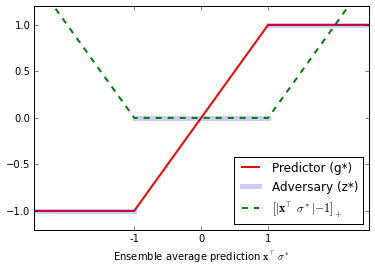
\includegraphics[width=0.55\textwidth]{figs/optstrats.png}
\caption{
\label{fig:optstrats}
The optimal strategies and slack function as a function of the ensemble prediction $\vx^\top \sigma^*$.}
\end{figure}

The proof of this theorem is a standard application of Lagrange duality and the minimax theorem.
The minimax value of the game and the optimal strategy for the predictor $\vg^*$ (Lemma~\ref{lem:game1gopt}) 
are our main objects of study and are completely characterized, 
and the theorem's partial description of $\vz^*$ (proved in Lemma \ref{lem:game1zopt}) 
will suffice for our purposes. 
\footnote{For completeness, Corollary \ref{cor:zoptfullpred} in the appendices 
specifies $z_i^*$ when $\abs{\vx_{i}^\top \sigma^*} = 1$.}

Theorem \ref{thm:gamesolngen} illuminates the importance of the optimal weighting $\sigma^*$ over hypotheses. 
This weighting $\sigma^* \in \argmin_{\sigma \geq 0^p} \gamma (\sigma)$ is the solution 
to a convex optimization problem (Lemma \ref{lem:helperthreshcvx}), 
and therefore we can efficiently compute it and $\vg^*$ to any desired accuracy. 
The ensemble prediction (w.r.t. this weighting) on the test set is $\vF^\top \sigma^*$, 
which is the only dependence of the solution on $\vF$. 

More specifically, the minimax optimal prediction and label \eqref{eqn:opt-strats} on any test set example $\vx_j$ 
can be expressed as functions of the ensemble prediction $\vx_j^\top \sigma^*$ 
on that test point alone, without considering the others. 
The $\vF$-dependent part of the slack function also depends separately on each test point's ensemble prediction. 
Figure \ref{fig:optstrats} depicts these three functions. 





\section{Ball Specialists}

We restrict our attention to a special case which corresponds,
roughly, to nearest neighbor methods.
\begin{enumerate}
  \item The input space is $R^d$.~\footnote{We use an arrow notation $\x$ to
    differentiate between $\x \in R^d$ and $\vx$ which denotes a row
    of the matrix $\vF$.}
    The rules that we use are ``specialists'' that are balls. The set
    $\B$ contains all rules of the form 
    \[
    B_{r,\cc,s}(\x) =
    \begin{cases}
      s & \text{if } \| \cc- \x \| \leq r \\
    0 & \text{otherwise }
    \end{cases}
    \]
    Where $r \geq 0$ is the radius of the ball, $\cc \in R^d$ is the
    center of the ball and $s \in \{-1,+1\}$ is the polarity of the ball.
    We will drop the subscripts of $B$ when clear from context.
  \item
    We use $\x \in B$ to indicate that $B(\x) \neq 0$.
  \item
    We denote by $\D$ the distribution of examples $(\x,y) \sim R^d
    \times \{-1,+1\}$.
  \item
    We denote the {\em probability} of a ball $B$ by $p(B) \doteq
    P_{\x \sim \D}(\x \in B)$
  \item
    We use the term {\em bias} of a ball to refer to the conditional
    expectation of the label for a ball by
    $$
    \bias(B) \doteq E_{(\x,y)\sim\D}\left( y|\x \in B \right)
    $$
\end{enumerate}




\newcommand{\edge}{\gamma}
\newcommand{\SepsGamSig}{\SS_{\epsilon,\edge}^{s}}
\newcommand{\SepsGam}{\SS_{\epsilon,\edge}}
\newcommand{\SepsGamMinusSig}{\SS_{\epsilon,\edge}^{-s}}
\newcommand{\ConstrepsGamSig}{\CC_{\epsilon,\edge}^{s}}
\newcommand{\ConstrepsGam}{\CC_{\epsilon,\edge}}
\newcommand{\ConstrepsGamMinusSig}{\CC_{\epsilon,\edge}^{-s}}

\section{Degrees of Safety}
We say that a point $\x$ is {\em safe} if we can confidently identify
the label of $\x$. We distinguish three levels of safety of
increasing strength: version-space (VS) safety, pairwise (PW) safety and
asymptotic (A) safety. We define each one in turn.

First, we need some notation. We denote the set of all balls by $\SS$. For any $\epsilon,\edge>0$
and $s \in \{-1,+1\}$ we define the set of $(\epsilon,\edge,s)$-
good balls $\SepsGamSig \subset \SS$ to be:
\[
\SepsGamSig \doteq \left\{B \in \SS \left| p(B) \geq \epsilon,
s\; \bias(B) > \edge \right. \right\}
\]
We define $\SepsGam^{\pm} \doteq \SepsGam^{+} \cup \SepsGam^{-}$

Denote by $V(\SepsGam^{\pm})$ the set of all point-wise biases $\vz$
that satisfy the constraints defined by $\SepsGam^{\pm}$

\begin{itemize}
\item {\bf Version space (VS) safety}\\
We are $(\epsilon,\edge,s)$-{\bf VS safe} on $\x$ if $s\sign(z(\x)) \geq 0$
for all $\vz$ that satisfy  $ \frac{1}{n} \vF \vz \geq \vb$.

\newcommand{\XepsGamSig}{\X_{\epsilon,\edge}^{s}}
\newcommand{\XepsGam}{\X_{\epsilon,\edge}}

\item
{\bf Pair-Wise (PW) safety}\\
We define the set of $(\epsilon,\edge,s)$-{\bf PW safe} instances
to be 
\[
\XepsGamSig \doteq \left\{\x \in R^d \left|
\begin{array}{l}
\exists B \in \SepsGamSig \mbox{ s.t. } \x \in B \mbox{ and } \\
\forall B \in \SepsGamMinusSig \mbox{ s.t. } \x \in B,\;\;
\exists B' \in \SepsGamSig \mbox{ s.t. } \x \in B' \mbox{ and } B'
\subset B
\end{array}
\right. \right\}
\]

\item
{\bf Asymptotic (A) Safety}\\ We say that $\x$ is $(\epsilon,\edge,s)$- {\bf A-safe} if
it is $(\epsilon,\gamma',s)$-{\bf PW safe} for all $0<\epsilon' \leq
\epsilon$ and $0<\gamma' \leq \gamma$ and for the same polarity $s$.
\end{itemize}


%We use $\XepsGam^{\pm}$ to denote $\XepsGam^{+} \cup \XepsGam^{-}$




\section{Rewriting the Constraint Set}

For the purposes of the analysis, it will often be useful to use the following fact. 
For any $(\epsilon,\edge,s)$-PW-safe point $ x $,
the constraint set can always be rewritten to contain no hypotheses predicting with the opposite polarity. 
This follows from the following simple fact.
\akshay{Please rewrite this if the notation is still not satisfactory. I went to the opposite extreme as last time, making it as general as possible.}

\begin{prop}
If for any functions of the labeling $a (\vz), b (\vz)$ we have constraints $a (\vz) + b (\vz) \leq 0$ and $a (\vz) \geq 0$, 
then $b (\vz) \leq 0$.
\end{prop}

In the definition of $PW$-safety, $a(\vz)$ corresponds to the masking (smaller) specialist $B'$, and $b(\vz)$ the complementary specialist that predicts on $B \setminus B'$ with the polarity of $B$.






\iffalse
\newcommand{\sol}{{\bf SOL}}


\newcommand{\erreg}{\err_{\epsilon,\gamma}}

With each polarity $s \in \{-1,+1\}$ and each ball
$B \in \SepsGam^s$ we associate a single constraint $s\; \bias(B) \geq b
\geq \gamma$. (We ignore the constraints that are an upper bound on
the bias). We denote the set of all constraints associated with
$\SepsGam^s$ by $\ConstrepsGam^s$.

For a point $\vx$ and a set of constraints $\CC$ we denote the optimal
solution of the min-max problem at the point $\x$ by $\vz^*(\x,\CC)$

\begin{lemma}
  Fix any $\epsilon,\gamma>0$, $s \in \{-1,+1\}$ and for all
  $\x \in \XepsGamSig$:
  \[
  \vz^*(\x,\ConstrepsGamSig) = \vz^*(\x,\ConstrepsGam^{\pm})
  \]
\end{lemma}
\yoav{There is still something missing from the proof. If
  $\vz^*(\x,\ConstrepsGam^{\pm})>0$. Then the effect of minimizing
    $\|\vz\|_1$ and the effect of any rule $(b,B) \in
    \ConstrepsGam^{-}$ is the same: it is to minimize $\vz(\x)$. So the
    removal of $(b,B)$ is truly redundant. However, it is possible
    that $\vz^*(\x,\ConstrepsGam^{\pm})=0$ in which case a more
      delicate argument is needed.}

\begin{proof}
  An alternative form of game~(\ref{game1eq}) is

\begin{align}
\displaystyle  \label{game2eq}
\vz^* = \argmin_{\substack{ \vz \in [-1,1]^n ,
    \\ \frac{1}{n} \vF \vz \in [\vb_l,\vb_u]}} \;\; \|\vz\|_1
\end{align}

Without loss of generality, set $s=+1$ and fix any $\x$.

Let $(B,b)$, $b<0$ be any element of $\ConstrepsGam^{-}$
such that $\x \in B$.

As $\x \in \XepsGam^{+}$, we know that there exists another ball
$(D,d) \in \ConstrepsGam^{+}$ such that $d>0$ and $\x \in D$ and $D \subset B$.

Define the variables $d',b'$ as
\[
d' \doteq \sum_{\y \in D} \vz^*(\y,\ConstrepsGam^{\pm})   \;\;\; b' \doteq \sum_{\y \in B} \vz^*(\y,\ConstrepsGam^{\pm})
\]
Using those we can write the conditions as
\[
d'\geq d \;\; \mbox{ and } b' \leq b
\]
Or alternatively, as
\[
d' \geq d \;\; \mbox{ and } b'-d' \leq b-d
\]
The second condition does not involve $\x$ so the removal of the condition $(B,b)$ from $\ConstrepsGam^{\pm}$ does not change the solution:
\[
\vz^*(\x,\ConstrepsGam^{\pm}) = \vz^*(\x,\ConstrepsGam^{\pm} \setminus \{(B,b)\} ) 
\]

As this holds simultaneously for all $(B,b) \in \ConstrepsGam^{-}$ the statement of the Lemma follows
\end{proof}
  
\section{Convergence}


\begin{assumption} The error $\erreg$ is well defined for all
  $\epsilon,\gamma>0$ and
  \[
  \lim_{\epsilon \to 0, \gamma \to 0} \erreg = \err^*
  \]
\end{assumption}






\section{Good Examples are Clipped}

Finally, we relate these definitions back to the slack function optimization problem. 
A definition that is useful is:
\begin{defn}
For $s = \pm 1$, define 
\begin{align*}
T_{\epsilon, \gamma}^{s} (\x) := \lrsetb{ B \in \SepsGam^{s} \mbox{ s.t. } \x \in B}
\end{align*}
\end{defn}

\subsection{Two Change-of-Basis Lemmas}

\begin{lemma}
\label{lem:replacespec}
Suppose the slack function over a set of specialists $\SepsGam^{s}$ is minimized by giving each example $x$ a score of $S^* (x)$. 
Take any $B \in \SepsGam^{s}$, and suppose that $\exists B' \in \SepsGam^{s} \mbox{ s.t. } B' \subset B \mbox{ and } B' (x) \neq B (x) \;\;\forall x \in B'$. 

Define the specialist $C$ predicting only on $B \setminus B'$ according to $B$. 
Then the slack function over the specialist class 
$$ \SepsGam^{s} \setminus \lrsetb{B} \cup \lrsetb{C} $$
has the same minimizer, with each example's score being $S^* (x)$. 
\end{lemma}
\begin{proof}
%It remains only to show that any $B \in T_{\epsilon, \gamma}^{s} (\x)$ can be replaced by a specialist predicting on $B \setminus B'$, without affecting the slack function optimum.
Note that $B'$ and $B$ influence the slack function only through the corresponding weights put on them by the algorithm $\sigma_{B'}, \sigma_{B} \geq 0$. 
Suppose the predictions of $B', B$ are $\vh_{B'}, \vh_{B} \in \RR^{n}$. 
Recall that $h_{B', i} = \frac{1}{p (B')} B' (x_i)$ where $B' (x_i) \in \lrsetb{-1, 0, 1}$. 
Then $B, B'$ are represented together in the optimization by $\sigma_{B'} \vh_{B'} + \sigma_{B} \vh_{B}$. 
This vector can be rewritten in terms of the two hypotheses $B'$ and $C$, where $C$ predicts according to $B$ on its domain $B \setminus B'$. 
\begin{align*}
\sigma_{B'} h_{B', i} + \sigma_{B} h_{B, i} 
&= \frac{\sigma_{B'}}{p (B')} B' (x_i) + \frac{\sigma_{B}}{p (B)} B (x_i) \\ 
&= \lrp{ \frac{\sigma_{B'}}{p (B')} - \frac{\sigma_{B}}{p (B)} } B' (x_i) \ifn(x_i \in B') + \frac{\sigma_{B}}{p (B)} B (x_i) \ifn(x_i \in B \setminus B') \\ 
&= \lrp{ \sigma_{B'} - \sigma_{B} \frac{p (B')}{p (B)} } h_{B', i} + \sigma_{B} \frac{p (C)}{p (B)} h_{C, i} 
\end{align*}
Thus optimizing with $\vh_{B'}$ and $\vh_{B}$ is equivalent to optimizing with $\vh_{B'}$ and $\vh_{C}$, and the conclusion follows.
\end{proof}

\begin{lemma}
\label{lem:replacesamesign}
For $s = \pm 1$, suppose the slack function over a set of specialists $\SepsGam^{s}$ is minimized by giving each example $x$ a score of $S^* (x)$. 
Take any $B, B' \in \SepsGam^{s}$ with the same polarity, 
and define the specialists $C, C'$ predicting with this polarity on $(B \Delta B'), (B \cap B')$ respectively. 
Then the slack function over the specialist class 
$$ \SepsGam^{s} \setminus \lrsetb{B, B'} \cup \lrsetb{C, C'} $$
has the same minimizer, with each example's score being $S^* (x)$. 
\end{lemma}
\begin{proof}
Similar to above.
\end{proof}

\subsection{Main Result}

\begin{lemma}
For any $\epsilon > 0, \gamma > 0, s = \pm 1$, take any $\x \in \XepsGamSig$. 
If $\sigma^* \geq \vzero^{\abs{\SepsGam^{s}}}$ is the minimizer of the slack function over good specialists $\SepsGam^{s}$, 
and $\x \in \RR^{\abs{\SepsGam^{s}}}$ is the vector of these specialists' predictions on $\x$, 
\begin{align}
s \x^\top \sigma^* \geq 1
\end{align}
\end{lemma}
\begin{proof}
For the given $\x$, by definition of $\XepsGamSig$, 
any $B \in T_{\epsilon, \gamma}^{-s} (\x)$ has a corresponding $B' \subset B$ such that $B' \in T_{\epsilon, \gamma}^{s} (\x)$. 
Lemma \ref{lem:replacespec} shows that the slack function problem is equivalent to one where $B$ is replaced in the ensemble by a specialist corresponding to $C := B \setminus B'$, 
which does not contain $\x$. 
Replacing each $B \in T_{\epsilon, \gamma}^{-s} (\x)$ in this way removes it from $T_{\epsilon, \gamma}^{-s} (\x)$ but conserves $T_{\epsilon, \gamma}^{s} (\x)$, 
to catalyze replacement of other elements of $T_{\epsilon, \gamma}^{-s} (\x)$. 
(Note that $C$ may not be in $\SepsGam^{s}$ because we could have $p(C) \leq \epsilon$.)
When all $B \in T_{\epsilon, \gamma}^{-s} (\x)$ are replaced, $T_{\epsilon, \gamma}^{-s} (\x)$ is empty, 
but $T_{\epsilon, \gamma}^{s} (\x)$ is identical, 
and contains all specialists in the new basis that predict on $\x$. 

Lemma \ref{lem:replacesamesign} shows that any intersecting pair of specialists in $T_{\epsilon, \gamma}^{s} (\x)$ can be replaced by three disjoint specialists of the same polarity without changing the minimization solution. 
Performing this replacement repeatedly, we eventually arrive at a basis in which exactly one specialist predicts on $x$, and potentially on other examples as well, for which it must be the only predictor. Call this specialist $h$.
Putting weight on $h$ will always lower the slack function if the examples in its support are hedged, proving the result.
\end{proof}

\akshay{Not sure about this because $h$ may have bias $< 0$ even though its parent specialists do not. }



\section{Intuition}
Here is some rough intuition.
One can think of $\SepsGam^{+}$ and $\SepsGam^{-}$ as competing teams
of specialists, those in the first team predict $+1$ (when they don't abstain)
while those in the other predict $-1$. Consider a particular point
$\x$, and consider subset of the specialists in $\SepsGam$ that
predict (i.e. do not abstain) on $\x$.

It is intuitively clear that if all of the predicting specialists
are members one team, that the solution $\sol$ will predict with the
same label as that team.

A less intuitive fact is that there are points for which there are
predictors from both teams but are still guaranteed to predict
according to one of the teams. These are the elements of
$\XepsGamSig$. Suppose $\sigma=+1$ and $\x \XepsGam^{+}$. There
might be specialists $B \in \SepsGam^{-}$such that $\x \in B$, but
for each such specialist there is another specialist $B' \in
\SepsGam^{+}$ such that $\x \in B'$ {\em and} $B' \subset
B$. Intuitively, the opinion of the more specialized specialist masks
the opinion of the more general one.

In terms of the game, the points in $\XepsGam$ are clipped points. I
am not sure whether points outside of $\XepsGam$ can also be clipped.

Predictions on $\x \in \XepsGam$ can change only if there is some
$\epsilon' \leq \epsilon$ and $\gamma'\leq \gamma$ such that for some 
$B \in \SS_{\epsilon',\gamma'}$ $B$ belongs to the opposite
team. Thus if we have reached the probability radius $\rho$ such that
for all $B$ where $\x \in B$ and $p(B)<\rho$ the sign of $B(vx)$ is
constant, we have reached the Bayes rule.

We can therefor call $\x \in \XepsGam$ the ``unknown unknown'', while
the complement of $\x$ are the ``known unknown''.







\section{From true dist to empirical}

Suppose now that we take a sample of $n$ points, and suppose that, at
each point of time, we have a sample of labels associated with
these points.

We can define the sets above relative to the empirical distribution
over $R^d$ but using the {\em true} distribution over the conditional
$p(y|\x)$.

Fixing $\epsilon$ and $\gamma$ we get, using uniform convergence, that
the empirical probability of all $B \in \SepsGam$ is bounded below by
$\epsilon/2$ and the bias is bounded below by $\gamma/2$

etc etc
\fi

\end{document}
